\begin{chapter}{\label{cha:intro}Introduction}

  \begin{center}
      \vfill
      \begin{redbox}
          \ \ \ \ \ \ \ \ \ \huge UNDER CONSTRUCTION!!!!!
          \normalsize
          \begin{enumerate}
              \item Background, motivating studies, and literature review?
              \item Actually dont like that idea.
              \item Background
              \begin{itemize}
                  \item $\rightarrow$ 
              \end{itemize}
              \item Motivating studies (I like the three `objectives' already written?)
              \item Literature review -- namely gap in the market?
              \item Thesis outline $\rightarrow$ should definitely be last thing.
          \end{enumerate}
      \end{redbox}
      \vfill
  \end{center}
  \clearpage

  \section{Thesis outline}
  % `Classic' methods -->
  In Chapter \ref{cha:methods-classic}, we lay the foundations for the thesis by first establishing the notation to be consistently used throughout. We then introduce the multivariate extension of the `classic' joint models \citep{Wulfsohn97, Henderson2000}, which are our specific models of interest. This  elucidates the parameters of interest as well as the estimation routine. Couched in a semiparametric maximum likelihood approach we provide an overview of the EM algorithm, aligning our methodology with  `classic' literature. Stemming from this approach, we introduce numerical integration methods. We further outline how one can `complete' inference and obtain standard errors for a fitted joint model. Finally, we offer a comprehensive overview of simulating data within the joint modeling framework; a crucial technique for the forthcoming chapters.

  In Chapter \ref{cha:approx}, we draw attention to the computational burden which precludes, or makes overtly cumbersome, estimation for multivariate joint models by maximum likelihood. We introduce a normal approximation first proffered by \citet{Bernhardt15}, allowing for the dimensionality of required integrals to be one; with exhaustive details of this approximate EM algorithm provided. This approximate EM algorithm is used exhaustively throughout the thesis. Extensive simulation results are given, which serve to showcase the performance of the algorithm. Additionally, we offer comparison in terms of computation time as well as parameter estimates with existing software which is similar in its estimation approach.

  In Chapter \ref{cha:flexible} we continue utilising the approximate EM algorithm but extend the longitudinal sub-model to the non-Gaussian case; the idea being that many clinical data will not be continuous, or the Gaussian assumption not otherwise appropriate. We consider five different exponential families and provide an overview of the estimation procedure required for these so-called `generalised' multivariate joint models in a similar spirit to Chapter \ref{cha:approx}. Once more we provide multitudes of simulation study results to exhibit performance of the approximate EM algorithm.

  Owing to its large-scale use in the thesis it is of considerable importance to thoroughly investigate, understand, and justify the normal approximation. In Chapter \ref{cha:justification}, beginning with its foundations before delineating strategies to justify said approximation, we seek to achieve this; swathes of results are provided along with interpretation.

  We then shift focus to avenues for analysis of a fitted joint model. That is, with the methodology outlined in Chapters \ref{cha:methods-classic}--\ref{cha:flexible}, what can one \textit{do} with the fitted joint model: Is it well behaved? How can it be used for predictions? Such questions are answered in Chapter \ref{cha:posthoc} where we collate post-hoc analyses, from defining residuals for the two processes, to outlining how one can bridge from a joint model to a predictive one.

  Chapter \ref{cha:app-PBC} can be viewed as something of an amalgamation of Chapters \ref{cha:methods-classic}, \ref{cha:approx}, \ref{cha:flexible}, and \ref{cha:posthoc}. We seek to provide an extensive application to a clinical set of data (primary biliary cirrhosis): The aim of the chapter is to identify, and perform post-hoc analyses on, the `best-fitting' (multivariate) joint model for this data.  

  Finally, the thesis is brought to a close by our conclusions along with discussions of possible future research avenues in Chapter \ref{cha:conclusion}. The thesis is supplemented by Appendices \ref{cha:appendix-ExtraStuff}--\ref{cha:appendix-supplementary-figures} which house an assortment of extra derivations and results (both tabulated and graphical). Finally Appendix \ref{cha:appendix-gmvjoint} provides a brief overview of the \tt{R} package built alongside the work in Chapter \ref{cha:flexible}, \tt{gmvjoint}, which is used to obtain \textit{all results} presented.
  
  \section{\label{sec:jointintro}Background to the joint modelling of survival and longitudinal data}
  In many areas of health research, collection of (potentially many) repeated measurements which are censored by a terminal event are commonplace. Interest then falls on the longitudinal trajectories, risk of event occurrence and the relationship between the two. The longitudinal response is assumed to be endogenous and is measured with error, which precludes inclusion in standard survival models as a time-varying covariate \citep{Prentice1982, Kalbfleisch2002}. The introduction of joint models allowed for simultaneous use of all longitudinal and survival information: When the longitudinal outcome and the time-to-event of interest are related, the modelling process must consider dropouts as non-random; dropout precludes further measurements of the longitudinal trajectories which could include information about the longitudinal process \citep{Martins2022}. Incorporation of the survival information into the longitudinal process has an equivalence to taking into account the effect of an informative missing data process. Conversely, incorporation of the longitudinal information into the survival process improves the fit of regression (i.e., reduces biases arising from separate model fits) and provides important inference on the relation between the event time and the longitudinal process.
  
  With specific interest then on characterising the relationship between the longitudinal response and the event-time, joint models are a popular modelling strategy. In essence, a joint model consists of (at least) two sub-models, which are linked by (at least) some shared random effects. Typically, a linear mixed model (LMM, \citet{LairdWare1982}) is used to describe the longitudinal response over time and a Cox proportional hazards (PH) model for the hazard of the event-time \citep{Cox1972}. The random effects in the LMM are then incorporated into the Cox PH model to capture the association between the longitudinal and event-time processes. Such a model specification allows for measurement error in the longitudinal covariates to be taken into account, therefore reducing bias that would arise from a separate analysis on the two sub-models \citep{Ibrahim2010}.
  
  \section{\label{sec:studies}Motivating studies}
  We briefly present three studies which motivate the usage of joint modelling. We further elucidate in Section \ref{sec:lit-early} that joint modelling itself arose due to analytical challenges found in the famous Burroughs-Wellcome HIV/AIDS trials which took place in the late 1980's, however we note that this data is not publicly available. Instead we highlight data which lends itself to joint modelling, and as such is commonly found in the literature. For all of the highlighted datasets, we can pose three questions of scientific interest which could be answered by such a joint analysis:
  \begin{enumerate}
      \item How do the biomarker(s) of interest evolve through time and differ in terms of the other covariates collected at baseline (e.g. drug allocation, sex)?
      \item How does the hazard for the endpoint of interest evolve through time and differ in terms of the other covariates collected at baseline?
      \item How is this hazard affected by underlying values of the biomarker(s) of interest?
  \end{enumerate}
   In these examples we focus on data arising from clinical trials on human subjects (although this is perhaps the traditional application of the Cox model). This isn't to say the relationships between longitudinal responses and an event-time of interest are \textit{only} of interest in a clinical setting; they will be of interest in other disciplines too.
  \subsection{\label{sec:motivation-pbc}Primary billiary cirrhosis}
   Primary billiary cirrhosis (PBC) is a chronic liver disease in which the bile ducts become injured, leading to a build-up of bile in the liver, which can damage it and lead to cirrhosis. If left untreated or otherwise reaches an advanced stage, PBC can lead to severe complications such as liver failure, hypertension and ultimately mortality. The progression of PBC was studied in 312 patients between 1974 and 1984 at the Mayo clinic \citep{PBCarticle}. In this study, the $312$ patients were randomised and received placebo ($n=154, 49.4\%$) or the active D-penicillamine. Several biomarkers associated with liver function were repeatedly measured during follow-up, as well as information regarding the time until the first occurrence of either death, receiving a transplantation, or end of study. The existence of multiple longitudinal biomarkers as well as information regarding a time to event of interest has led to the PBC data becoming a popular example in existing literature \citep{Hickey2018, PBCapp1, PBCapp2, PBCapp3}. The longitudinal trajectories of three biomarkers, serum bilirubin (measured in log mg/dL), albumin (measured in g/dL) and prothrombin time (blood clotting time, measured in seconds) are presented in Figure \ref{fig:PBCtrajectories} amongst patients who experienced mortality. These could lead one to hypothesise that lower values of albumin or prothrombin increase the risk of mortality, with the same true for higher values of serum bilirubin.
  
  \begin{figure}[h]
      \centering
      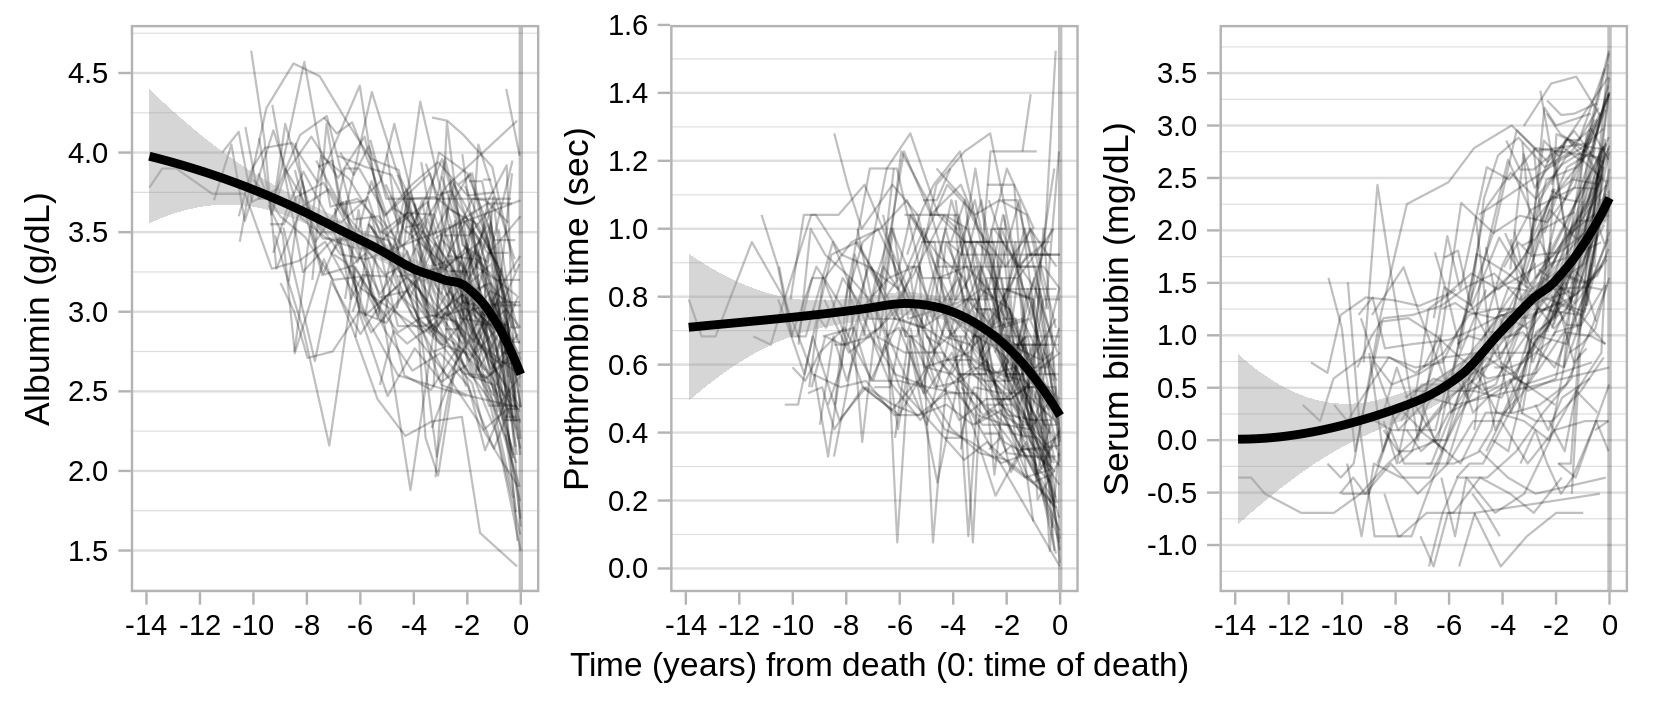
\includegraphics[width=140mm, height=60mm]{Figures/PBCtrajectories.png}
      \caption{Longitudinal trajectories for the three chosen biomarkers from PBC data. The black lines show individual trajectories and the thick line shows a smoothed (LOESS) curve along with a shaded band representing the 95\% confidence interval.}
      \label{fig:PBCtrajectories}
  \end{figure}
  
  \subsection{\label{sec:motivation-adni}Alzheimer's disease neuroimaging initiative (ADNI)}
  The Alzheimer's Disease Neuroimaging Initiative 1 (ADNI-1, henceforth `ADNI') study (\url{http://adni.loni.ucla.edu/}) is a prospective cohort study which began in 2004. More than 800 individuals were recruited with differing levels of cognitive impairment (cognitively normal, mild impairment and early Alzheimer's), of which we solely focus on those who were mildly cognitively impaired at baseline. The subjects of the study re-attended across three years (provisionally) of follow-up. Numerous biomarkers were collected throughout this time: Neuropsychological assessments; brain imaging and other clinical measures along with time until conversion to Alzheimer's Disease (the end-point of interest, `AD').\newline Previous work essentially `ranked' all collected biomarkers by their predictive capabilities from a series of univariate joint model fits (\cite{Li2017A}, Tables 2--3). Figure \ref{fig:ADNItrajectories} illustrates the longitudinal trajectories of the three best-performing biomarkers identified in \cite{Li2017A}: The Alzheimer’s Disease Assessment Scale-Cognitive subscale (13 item, ‘ADAS-13’); Functional assessment questionnaire (‘FAQ’) and MRI volumetric data of the middle temporal gyrus, which were identified as the best-performing biomarkers in the cognitive, functional and neuroimaging domains, respectively. These plots may lead us to posit that increased (e.g. above average) scores in either ADAS-13 or FAQ assessments -- both of which indicate greater functional dependence -- lead to increased hazard of conversion to Alzheimer's Disease, and the opposite being true for volumetric reading of the middle temporal gyrus, although the hazard here may not be as greatly influenced.
  
  \begin{figure}[t]
      \centering
      \includegraphics[width = 140mm, height = 60mm]{Figures/ADNItrajectories.png}
      \caption{Longitudinal trajectories for ADAS-13; FAQ and middle temporal gyrus volume from the subset of the ADNI data who experienced AD conversion. Black lines show individual trajectories and the thick black line shows a smoothed (LOESS) curve along with a shaded band representing the 95\% confidence interval.}
      \label{fig:ADNItrajectories}
  \end{figure}
  
  \subsection{\label{sec:motivation-kidney}Chronic kidney disease}
  Chronic kidney disease (or, chronic renal disease), is the progressive loss of renal function over a period of time. During a study conducted between 1983 and 2000, 407 patients who had undergone renal transplantation with a graft from a donor had the long-term performance of their new graft assessed and the time to failure of the new graft also measured. The performance of the patient's kidneys was assessed through repeated collection of biomarkers. For brevity we focus on the same three chosen in existing literature \citep{Rizopoulos2011B}: Glomerular filtration rate (GFR), which measures filtration rate of the kidneys; proteinuria  that measures whether the kidneys succeed in sustaining the proteins in the blood and not discard them in the urine (thus a binary covariate); and the blood haematocrit level that measures whether the kidneys produce adequate amounts of the hormone that regulates the red blood cell production. The longitudinal profiles of the continuous biomarkers (i.e. GFR and blood haematocrit level) amongst those whose kidney transplantation failed during follow-up ($n=126, 31.0\%)$ is presented in Figure \ref{fig:Kidneytrajectories}. 
  
  \begin{figure}[h]
      \centering
      \includegraphics[height=60mm, width=140mm]{Figures/KidneyContinuousTrajectories.png}
      \caption{Longitudinal trajectory of the two continuous biomarkers routinely collected during kidney graft study: Blood haematocrit and glomerular filtration rate (GFR). The trajectories shown here are subjects whose kidney graft failed. Black lines show individual trajectories and the thick black line shows a smoothed (LOESS) curve along with a shaded band representing the 95\% confidence interval.}
      \label{fig:Kidneytrajectories}
  \end{figure}
  
  This figure allows us to infer, particularly for GFR that a deviation away from the average trajectory (i.e. a lower value) increases the hazard of kidney graft failure. Figure \ref{fig:Kidneyprot} illustrates the status of this binary biomarker for subjects whose proteinurea status changed more than 25 during follow-up and ultimately experienced graft failure. The figure perhaps suggests that one is more likely to have a failed kidney graft if proteinurea is consistently present. The use of generalised linear mixed models in a joint modelling context is explored in detail in Section \ref{sec:lit-glmm}.
  
  \begin{figure}[t]
      \centering
      \includegraphics[height=60mm, width=140mm]{Figures/KidneyBinaryTrajectories.png}
      \caption{Time series plot for binary biomarker proteinurea amongst those whose kidney graft failed and whose proteinurea status changed more than twenty-five times during follow-up. `ID' is a dummy ID amongst those the above is true for.}
      \label{fig:Kidneyprot}
  \end{figure}
  
  \section{\label{sec:lit}Literature review}
  We begin by establishing what caused the rise of joint models in literature: What issues arose through the use of the preceding, na\"{i}ve methods, and what were the `stepping stones' that brought around the advent of joint models as they were first introduced.
  \subsection{\label{sec:lit-early}How did we get here? An overview of precursory methodology}
  \subsubsection*{Early motivation and a na\"{i}ve approach}
  \addtocounter{subsubsection}{1}
  Much of the early contributions to the field of joint modelling was motivated by problems arising from HIV/AIDS research, although the issues are commonplace across many e.g. clinical trials where covariate information is repeatedly collected along with information relating to an event time of interest such as death. Covariates here are measured only intermittently and with some error. Suppose we want to know how the longitudinal trajectories affected the hazard in the Cox PH model. A na\"{i}ve approach would be to simply include the biomarker(s) as time-dependent covariate(s) in a Cox PH regression model \citep{Andersen1982}. However, such an approach ignores the fact that the biomarker are measured with error, and \citet{Prentice1982} showed that the presence of this random error causes parameter estimates obtained from subsequent model fits to be biased towards the null, thus any true association between the covariate trajectory and the response will be underestimated \citep{Sweeting2011}. Additionally, such an approach does not model the longitudinal profile itself, which will be of at least some tertiary interest.
  
  \subsubsection*{A two-stage approach}
  \addtocounter{subsubsection}{1}
  Improvements over this na\"{i}ve approach followed. With so-called two-stage models, having an emergence in the literature in the 1990s. Both \citet{Tsiatis1995} and \citet{DeGruttola1994} present this approach along with an application to aforementioned HIV/AIDS data, albeit with slight reparameterisation of the survival process in the latter example. Essentially, under the two-stage methodology, instead of modelling the covariates directly, the longitudinal process is first modelled separately using standard techniques (e.g. \citet{LairdWare1982}) and the best linear unbiased predictors of the random effects extracted. Subsequently in the second `stage', these random effects are used as time-varying covariates in the Cox PH regression model as previously described.\\ 
  Immediate advantages to this approach are the reduced bias obtained in parameter estimates \citep{Dafni1998} in comparison with na\"{i}ve methods, and the first stage allows for flexible specification of the random effects \citep{Bycott1998}. Additionally, these two-stage models are relatively easy to implement. However, the approach does not account for informative dropout, which could indicate violations surrounding the normality of the random effects will ensue \citep{Wulfsohn97, JMOverview}, nor does it incorporate observed survival information in modelling the covariate process, and so information is not wholly efficiently used \citep{Wulfsohn97}. In addition, compared to joint models which follow, parameter estimates also suffer bias \citep{Ibrahim2010}.\\
  Ultimately then, the two-stage model provided -- under no uncertain terms -- an improvement over the na\"{i}ve approach, but the methodology was not optimal, for reasons given above.
  
  \subsection{Joint modelling}
  \subsubsection*{A Bayesian antecedent}
  \addtocounter{subsubsection}{1}
  The stage is now set for joint models as described in Section \ref{sec:jointintro} to arise. We first mention in passing early efforts conducted under a Bayesian hierarchical framework, namely \citet{Berzuini1996} and \citet{Faucett1996}. Given these early efforts pre-dated standard software such as \tt{WinBUGS} \citep{Winbugs-manual}, they employ tailor-made Gibbs sampling to estimate the posterior distribution of the unknown parameters. \citet{Sweeting2011} elucidate more on the early Bayesian efforts, and detail performance. Perhaps owing to the absence of widely available user-friendly software -- or because of clinicians typically operating under the frequentist paradigm -- these early Bayesian approaches perhaps appear to be secondary to the seminal paper introducing joint modelling by \citet{Wulfsohn97} in hindsight.
  
  \subsubsection*{A seminal paper and subsequent extensions}
  \addtocounter{subsubsection}{1}
  \citet{Wulfsohn97} introduced the simultaneous modelling of longitudinal and time-to-event data using maximum likelihood estimation via the Expectation Maximisation (EM) algorithm \citep{Dempster77}. The paper by \citet{Wulfsohn97} utilised low-dimensional Gauss-Hermite quadrature to approximate necessary expectations required for formulating the maximum likelihood estimates at each iteration of the EM algorithm. 
  
  \citet{Wulfsohn97} demonstrated their approach using a simplified model containing only the random effects in an application to the oft-considered HIV/AIDS data, wherein the parameter estimates obtained were shown to be similar when compared to a two-stage model. \citet{Tsiatis1995}; \citet{Faucett1996}; \citet{Bycott1998}; \citet{Dafni1998} and \citet{Wulfsohn97} all assumed bivariate Gaussian random effects in the form of an intercept and slope structure when approaching this data application. \citet{Henderson2000} extend the EM algorithm for joint modelling provided by \citet{Wulfsohn97} in specifying a stationary Gaussian process as part of the random effects structure (this was also the specification in \citet{Xu2001}, who instead opt for MCMC schemes), and \citet{Wang2001} provide an example of using a non-stationary Gaussian process. \citet{Henderson2000} additionally utilise antithetic Monte Carlo sampling, due to apparent computational inefficiency under proposed quadrature in their E-step, which set something of a precedent going forward.

  Competing risks sub-models are additionally a -- fairly obvious -- extension given the underlying Cox model. A joint model with a competing risks survival sub-model \citep{Williamson2008, Li2010} would be more useful in circumstances where patients can experience multiple events of interest: For instance death or disease recurrence; recurrent events such as re-admission to hospital; or a succession of events such as transition between (e.g. worsening of) disease states \citep{Hickey2018B}. Additionally, joint frailty-copula models have undergone something of a recent surge in popularity \citep{Emura2017, Peng2018, Sofeu2021}.
  
  \subsection{Evolution}
  
  \subsubsection*{\label{sec:lit-glmm}Generalised linear mixed models}
  \addtocounter{subsubsection}{1}
  Joint models with a continuous longitudinal response are ubiquitous in the literature. However, it is unlikely that every longitudinal response one measures in e.g. health research are best represented as a continuous (i.e. Gaussian) response. For instance, it could be of importance to identify the status of a specific event which can vary over time, with its presence or absence thought to be related to survival. Likewise, data which is either bounded or takes the form of an integer (or both) would likely better suit a count regression sub-model. Of course, one could standardise responses of interest such that residuals satisfy the usual assumptions, but this comes at the cost of model interpretability, which likely would preclude wider clinical uptake.\newline
  The emergence of joint models with (at least one) non-Gaussian sub-model is therefore not surprising. These can arise in two (not necessarily exclusive) ways. The first replaces the survival sub-model with a generalised linear model (GLM): When occurrence of an event of interest is more important than the timing of said event, then the proportional hazards model is replaced by a binary (i.e. logistic) sub-model. Examples include primary endpoints of successful pregnancy \citep{Horrocks2009}; survival past a certain period of follow-up \citep{Bernhardt15}; diagnosis of orthostatic hypertension with a single longitudinal response \citep{Hwang2011} and multiple longitudinal responses \citep{Hwang2015}; and diagnosis of late-life major depressive disorder, which was investigated under a Bayesian paradigm with competing link functions \citep{li2015flexible}.\newline 
  The second replaces (at least one) longitudinal sub-model with a generalised linear mixed model (GLMM): In circumstances where a longitudinal response cannot be cast in the `classic` Gaussian framework, such that a simple LMM is not appropriate, instead replaced by a suitable member of the exponential family and modeled by a GLMM. When the response is repeatedly measured and scored against a Likert-type scale, (partial) proportional odds models could be used \citep{Li2010, Alam2021}. Additionally, \citet{He2013} model cumulative probabilities of an ordianl outcome as part of a multivariate joint model also including a longitudinal binary response. Indeed, a biomarker of interest could take the form of a longitudinal binary response, in which case its longitudinal sub-model GLMM would take the form of a logistic one. Examples of this include \citet{Choi2015} who include repeated quality of life (1=satisfied) measures and \citet{Rustand2023} who include presence of malformed blood vessels in their analysis of the PBC data outlined in Section \ref{sec:motivation-pbc} in their multivariate longitudinal specification. Finally, the longitudinal response may be best represented by a count regression model. \citet{Sunethra2018} present a joint model with the number of seizures experienced by epilepsy patients captured by a Poisson GLMM sub-model and the time to first seizure post-randomisation. \citet{Zhu2018} utilise a zero-inflated Poisson (and generalised Poisson) GLMM in modelling daily cigarette count along with time to study dropout. \citet{Hickey2016} provide a good overview of usage of GLMM sub-models in joint modelling.

  \subsubsection*{\label{sec:lit-mv}The multivariate case} 
  \addtocounter{subsubsection}{1}
  When more than one longitudinal response is believed to be associated with the hazard of the event of interest -- and the multiple longitudinal responses are correlated with one another -- then harnessing all available information in a single joint model (rather than a series of univariate fits) would be advantageous. As alluded to fleetingly in the previous section these models with more than one longitudinal response constructing the longitudinal sub-model along with a survival sub-model are referred to as \textit{multivariate} joint models. In literature, such joint models were originally restricted to methodological developments \citep{Lin2002}. Only recently has software development allowed for routine fitting of joint models with potentially many longitudinal responses. These include likelihood-based approaches such as \tt{R} package \tt{joineRML} \citep{Hickey2018} and Markov Chain Monte Carlo (MCMC) methods in \tt{JMbayes2} \citep{R-JMbayes2}.\newline
  Multivariate joint models are superior to multiple univariate fits as they take into account the aforementioned correlation between the longitudinal responses of interest. Both \citet{Andrinopoulou2020} and \citet{Long2018} employ multivariate joint models, where the longitudinal sub-model is wholly constructed by LMMs (i.e. the responses are all treated as Gaussian), which is fit under the Bayesian paradigm by MCMC methods. Conversely, \citet{Hickey2018} and \citet{Philipson2020} multivariate joint models constructed by LMMs are fit using maximum likelihood. \citet{PBCapp2} utilise a Bayesian approach with shrinkage priors to fit a multivariate joint model, whose longitudinal specification includes GLMMs; \citet{Rustand2023} fit a similarly specified model using Integrated Nested Laplace Approximations (INLA, \citet{R-INLA}).\newline
  Even in light of developments of \tt{R} packages which allow fitting of multivariate joint models, in existing literature a common approach is to use dimension reduction techniques, such as functional principal components regression \citep{Li2017B, Li2021} or partial least squares \citep{Wang2020}. These approaches which utilise dimension reduction techniques are largely in scenarios where very many longitudinal responses exist (e.g. the ADNI data explored in Section \ref{sec:motivation-adni}), and existing methods do not allow for fitting such rich longitudinal specifications. Indeed, \citet{Hickey2018} hypothesised that an approximate method would be necessary to tackle issues which arise -- regardless of computational approach -- when rich sub-models are considered. \citet{Bernhardt15} introduced one such approximation, which we explore in great detail in Chapter \ref{cha:approx}.

\subsubsection*{\label{sec:lit-software}Available software to fit joint models}
\addtocounter{subsubsection}{1}
  Initially, uptake of joint models in e.g. clinical application was slow \citep{Gould2015}. One could argue that this was due to familiarity with long-existing methods (i.e. Cox models), despite the proven superiority of joint models, which also shared the same interpretation. Of course, a facet which would prohibit uptake of any methodology would be access to (or indeed lack thereof) readily available packages/libraries implemented in popular statistical software. We briefly note implementation of joint modelling in Statistical software \tt{Stata} through package \tt{stjm} \citep{stata-stjm}, as well as usage of \tt{SAS} to fit joint models through macro \tt{\%JM} \citep{SAS-JM}, and continue instead with a focus on \tt{R} \citep{R-R} packages available on the comprehensive R archive network (CRAN, \url{https://cran.r-project.org/}). \citet{Furgal2019} offer a comprehensive review and comparison via simulation studies of \tt{R} packages \tt{JM} \citep{R-JM}; \tt{joineR} \citep{R-joineR} and \tt{JMbayes} \citep{R-JMbayes}. We note that the authors do not consider multivariate joint models, which we detail in Section \ref{sec:lit-mv}. \newline
  The broad spectrum of available packages are perhaps reflective of phenomena within joint modelling. The first is the numerous functional forms one can implements -- many of which reflect ones prior beliefs -- in inducing an association between the longitudinal and survival sub-models as well as on the baseline hazard. Secondly, when \citet{Wulfsohn97} introduced joint modelling, they did so using low-dimensional quadrature, which do not scale well when more complex models are considered. This computational infeasibility lead to the use of Monte Carlo techniques \citep{Henderson2000, Lin2002, Hickey2018} as well as MCMC methods \citep{Rizopoulos2009, PBCapp3} to circumvent supreme computational burden. Thirdly, and perhaps most cogent in light of packages which are `sequels', is the technological advancements -- particularly in home computing power -- which allow for integration of \tt{R} and many fast and powerful libraries, such as with \tt{C++} \citep{R-Rcpp} as well as fast matrix algebra libraries such as Armadillo \citep{R-RcppArmadillo} and fast MCMC approaches \citep{R-stanjm}.

\end{chapter}